\documentclass{standalone}
\usepackage{tikz}
\usetikzlibrary{patterns, positioning}

\begin{document}
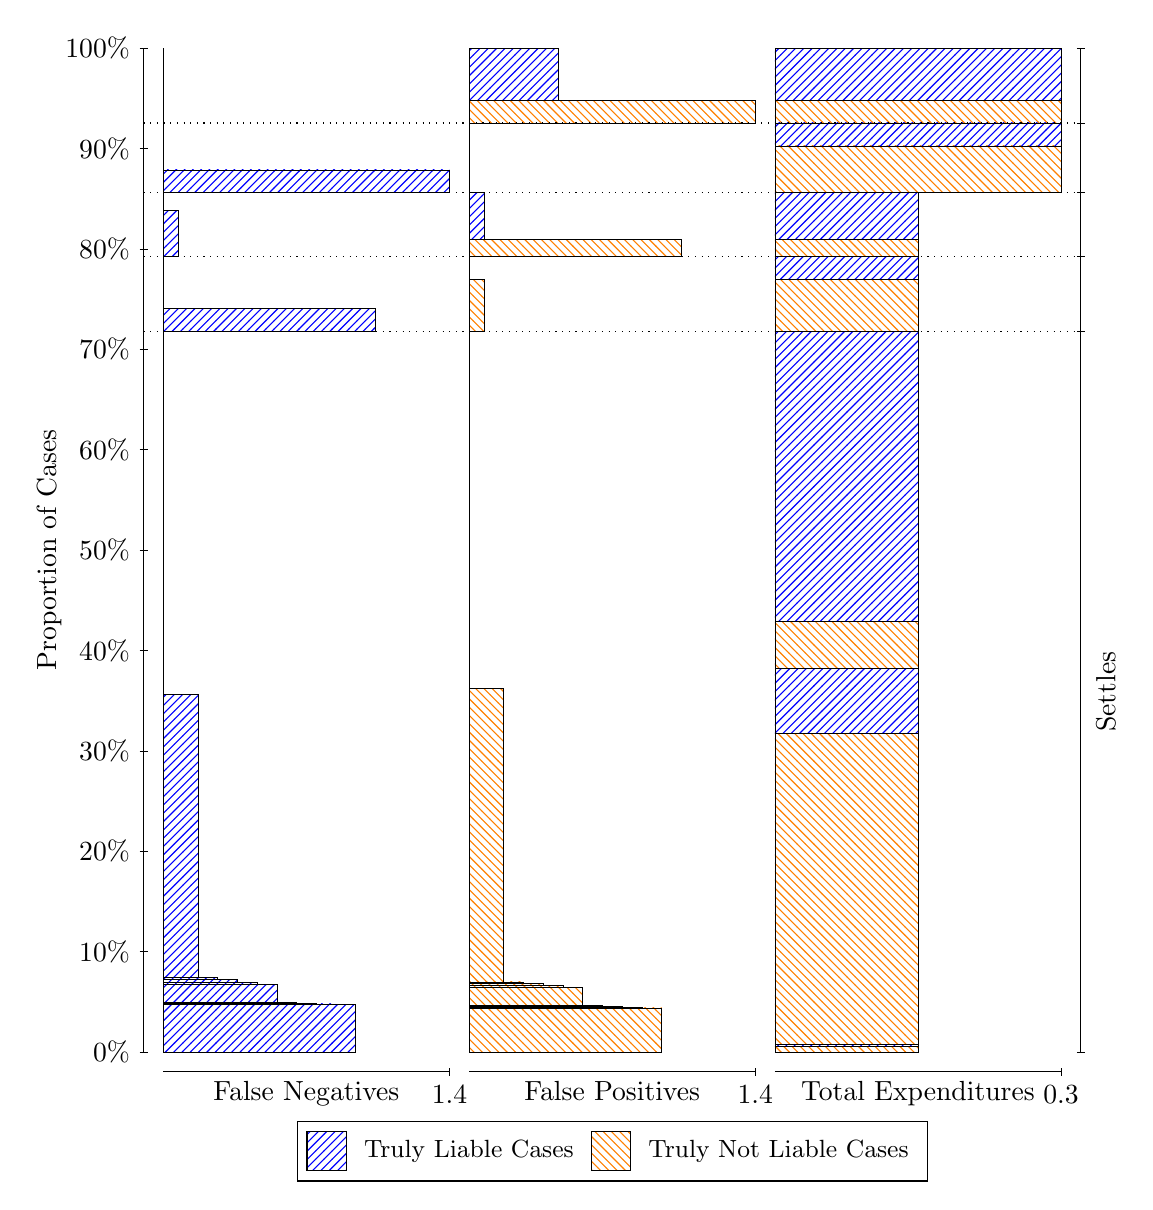
\begin{tikzpicture}
\draw[black, very thin] (1.5,1.75) -- (1.5,14.5);
\node[rotate=90, anchor=center] at (0.3, 8.125) {Proportion of Cases};
\draw[black, very thin] (1.45,1.75) -- (1.55,1.75);
\node[anchor=east] at (1.45, 1.75) {0\%};
\draw[black, very thin] (1.45,3.025) -- (1.55,3.025);
\node[anchor=east] at (1.45, 3.025) {10\%};
\draw[black, very thin] (1.45,4.3) -- (1.55,4.3);
\node[anchor=east] at (1.45, 4.3) {20\%};
\draw[black, very thin] (1.45,5.575) -- (1.55,5.575);
\node[anchor=east] at (1.45, 5.575) {30\%};
\draw[black, very thin] (1.45,6.85) -- (1.55,6.85);
\node[anchor=east] at (1.45, 6.85) {40\%};
\draw[black, very thin] (1.45,8.125) -- (1.55,8.125);
\node[anchor=east] at (1.45, 8.125) {50\%};
\draw[black, very thin] (1.45,9.4) -- (1.55,9.4);
\node[anchor=east] at (1.45, 9.4) {60\%};
\draw[black, very thin] (1.45,10.675) -- (1.55,10.675);
\node[anchor=east] at (1.45, 10.675) {70\%};
\draw[black, very thin] (1.45,11.95) -- (1.55,11.95);
\node[anchor=east] at (1.45, 11.95) {80\%};
\draw[black, very thin] (1.45,13.225) -- (1.55,13.225);
\node[anchor=east] at (1.45, 13.225) {90\%};
\draw[black, very thin] (1.45,14.5) -- (1.55,14.5);
\node[anchor=east] at (1.45, 14.5) {100\%};

\draw[black, very thin] (13.4,1.75) -- (13.4,14.5);
\draw[black, very thin] (13.35,1.75) -- (13.45,1.75);
\node[anchor=west] at (13.35, 1.75) {};
\draw[black, very thin] (13.35,10.903) -- (13.45,10.903);
\node[anchor=west] at (13.35, 10.903) {};
\draw[black, very thin] (13.35,11.849) -- (13.45,11.849);
\node[anchor=west] at (13.35, 11.849) {};
\draw[black, very thin] (13.35,12.662) -- (13.45,12.662);
\node[anchor=west] at (13.35, 12.662) {};
\draw[black, very thin] (13.35,13.548) -- (13.45,13.548);
\node[anchor=west] at (13.35, 13.548) {};
\draw[black, very thin] (13.35,14.5) -- (13.45,14.5);
\node[anchor=west] at (13.35, 14.5) {};

\draw[black, very thin, pattern color=blue, pattern=north east lines] (1.75,1.75) rectangle (4.1931,2.3508);
\draw[black, very thin, pattern color=blue, pattern=north east lines] (1.75,2.3508) rectangle (3.9425,2.36);
\draw[black, very thin, pattern color=blue, pattern=north east lines] (1.75,2.36) rectangle (3.692,2.3702);
\draw[black, very thin, pattern color=blue, pattern=north east lines] (1.75,2.3702) rectangle (3.4414,2.3806);
\draw[black, very thin, pattern color=blue, pattern=north east lines] (1.75,2.3806) rectangle (3.1908,2.6068);
\draw[black, very thin, pattern color=blue, pattern=north east lines] (1.75,2.6068) rectangle (2.9402,2.6372);
\draw[black, very thin, pattern color=blue, pattern=north east lines] (1.75,2.6372) rectangle (2.6897,2.6678);
\draw[black, very thin, pattern color=blue, pattern=north east lines] (1.75,2.6678) rectangle (2.4391,2.698);
\draw[black, very thin, pattern color=blue, pattern=north east lines] (1.75,2.698) rectangle (2.1885,6.2895);
\draw[black, very thin, pattern color=orange, pattern=north west lines] (1.75,6.2895) rectangle (1.75,10.903);
\draw[black, very thin, pattern color=blue, pattern=north east lines] (1.75,10.903) rectangle (4.4437,11.194);
\draw[black, very thin, pattern color=orange, pattern=north west lines] (1.75,11.194) rectangle (1.75,11.849);
\draw[black, very thin, pattern color=blue, pattern=north east lines] (1.75,11.849) rectangle (1.9379,12.442);
\draw[black, very thin, pattern color=orange, pattern=north west lines] (1.75,12.442) rectangle (1.75,12.662);
\draw[black, very thin, pattern color=blue, pattern=north east lines] (1.75,12.662) rectangle (5.3833,12.952);
\draw[black, very thin, pattern color=orange, pattern=north west lines] (1.75,12.952) rectangle (1.75,13.548);
\draw[black, very thin, pattern color=orange, pattern=north west lines] (1.75,13.548) rectangle (1.75,13.838);
\draw[black, very thin, pattern color=blue, pattern=north east lines] (1.75,13.838) rectangle (1.75,14.5);
\draw[black, very thin, pattern color=orange, pattern=north west lines] (5.6333,1.75) rectangle (8.0764,2.3086);
\draw[black, very thin, pattern color=orange, pattern=north west lines] (5.6333,2.3086) rectangle (7.8259,2.3207);
\draw[black, very thin, pattern color=orange, pattern=north west lines] (5.6333,2.3207) rectangle (7.5753,2.3336);
\draw[black, very thin, pattern color=orange, pattern=north west lines] (5.6333,2.3336) rectangle (7.3247,2.3462);
\draw[black, very thin, pattern color=orange, pattern=north west lines] (5.6333,2.3462) rectangle (7.0741,2.5684);
\draw[black, very thin, pattern color=orange, pattern=north west lines] (5.6333,2.5684) rectangle (6.8236,2.5691);
\draw[black, very thin, pattern color=orange, pattern=north west lines] (5.6333,2.5691) rectangle (6.8236,2.5931);
\draw[black, very thin, pattern color=orange, pattern=north west lines] (5.6333,2.5931) rectangle (6.573,2.6171);
\draw[black, very thin, pattern color=orange, pattern=north west lines] (5.6333,2.6171) rectangle (6.3224,2.6399);
\draw[black, very thin, pattern color=orange, pattern=north west lines] (5.6333,2.6399) rectangle (6.0718,6.3633);
\draw[black, very thin, pattern color=blue, pattern=north east lines] (5.6333,6.3633) rectangle (5.6333,10.903);
\draw[black, very thin, pattern color=orange, pattern=north west lines] (5.6333,10.903) rectangle (5.8213,11.558);
\draw[black, very thin, pattern color=blue, pattern=north east lines] (5.6333,11.558) rectangle (5.6333,11.849);
\draw[black, very thin, pattern color=orange, pattern=north west lines] (5.6333,11.849) rectangle (8.327,12.07);
\draw[black, very thin, pattern color=blue, pattern=north east lines] (5.6333,12.07) rectangle (5.8213,12.662);
\draw[black, very thin, pattern color=orange, pattern=north west lines] (5.6333,12.662) rectangle (5.6333,13.258);
\draw[black, very thin, pattern color=blue, pattern=north east lines] (5.6333,13.258) rectangle (5.6333,13.548);
\draw[black, very thin, pattern color=orange, pattern=north west lines] (5.6333,13.548) rectangle (9.2667,13.838);
\draw[black, very thin, pattern color=blue, pattern=north east lines] (5.6333,13.838) rectangle (6.7609,14.5);
\draw[black, very thin, pattern color=orange, pattern=north west lines] (9.5167,1.75) rectangle (11.333,1.8215);
\draw[black, very thin, pattern color=blue, pattern=north east lines] (9.5167,1.8215) rectangle (11.333,1.8512);
\draw[black, very thin, pattern color=orange, pattern=north west lines] (9.5167,1.8512) rectangle (11.333,5.7968);
\draw[black, very thin, pattern color=blue, pattern=north east lines] (9.5167,5.7968) rectangle (11.333,6.6239);
\draw[black, very thin, pattern color=orange, pattern=north west lines] (9.5167,6.6239) rectangle (11.333,7.2201);
\draw[black, very thin, pattern color=blue, pattern=north east lines] (9.5167,7.2201) rectangle (11.333,10.903);
\draw[black, very thin, pattern color=orange, pattern=north west lines] (9.5167,10.903) rectangle (11.333,11.558);
\draw[black, very thin, pattern color=blue, pattern=north east lines] (9.5167,11.558) rectangle (11.333,11.849);
\draw[black, very thin, pattern color=orange, pattern=north west lines] (9.5167,11.849) rectangle (11.333,12.07);
\draw[black, very thin, pattern color=blue, pattern=north east lines] (9.5167,12.07) rectangle (11.333,12.662);
\draw[black, very thin, pattern color=orange, pattern=north west lines] (9.5167,12.662) rectangle (13.15,13.258);
\draw[black, very thin, pattern color=blue, pattern=north east lines] (9.5167,13.258) rectangle (13.15,13.548);
\draw[black, very thin, pattern color=orange, pattern=north west lines] (9.5167,13.548) rectangle (13.15,13.838);
\draw[black, very thin, pattern color=blue, pattern=north east lines] (9.5167,13.838) rectangle (13.15,14.5);
\draw[black, dotted] (1.5,10.903) -- (13.4,10.903);
\draw[black, dotted] (1.5,11.849) -- (13.4,11.849);
\draw[black, dotted] (1.5,12.662) -- (13.4,12.662);
\draw[black, dotted] (1.5,13.548) -- (13.4,13.548);
\draw[black, very thin] (1.75,1.5) -- (5.3833,1.5);
\node[anchor=north] at (3.5667, 1.5) {False Negatives};
\draw[black, very thin] (5.3833,1.45) -- (5.3833,1.55);
\node[anchor=north] at (5.3833, 1.45) {1.4};

\draw[black, very thin] (5.6333,1.5) -- (9.2667,1.5);
\node[anchor=north] at (7.45, 1.5) {False Positives};
\draw[black, very thin] (9.2667,1.45) -- (9.2667,1.55);
\node[anchor=north] at (9.2667, 1.45) {1.4};

\draw[black, very thin] (9.5167,1.5) -- (13.15,1.5);
\node[anchor=north] at (11.333, 1.5) {Total Expenditures};
\draw[black, very thin] (13.15,1.45) -- (13.15,1.55);
\node[anchor=north] at (13.15, 1.45) {0.3};

\node[black, centered, rotate=90] at (13.72, 6.3264) {Settles};





\draw (7.449999999999999,1.5) node[draw=none] (baseCoordinate) {};
\begin{scope}[align=center]
        \matrix[scale=0.5, draw=black, below=0.5cm of baseCoordinate, nodes={draw}, column sep=0.1cm]{
            \node[rectangle, draw, minimum width=0.5cm, minimum height=0.5cm, pattern=north east lines, pattern color=blue] {}; &
            \node[draw=none, font=\small] (B) {Truly Liable Cases}; &
            \node[rectangle, draw, minimum width=0.5cm, minimum height=0.5cm, pattern=north west lines, pattern color=orange] {}; &
            \node[draw=none, font=\small] (B) {Truly Not Liable Cases}; \\
            };
\end{scope}

\end{tikzpicture}
\end{document}